\documentclass[aspectratio=169,10pt]{beamer}

\usetheme{default}
\usecolortheme{default}
\setbeamertemplate{navigation symbols}{}
\setbeamertemplate{footline}[frame number]
\setbeamercolor{structure}{fg=black}
\setbeamercolor{title}{fg=black}
\setbeamercolor{frametitle}{fg=black}
\setbeamerfont{frametitle}{series=\bfseries,size=\large}
\setbeamerfont{title}{series=\bfseries,size=\Large}

\usepackage{booktabs}
\usepackage{graphicx}
\usepackage{microtype}
\usepackage{tikz}
\usetikzlibrary{arrows.meta,positioning,fit,calc}
\setlength{\leftmargini}{1.2em}
\setlength{\itemsep}{0.28em}

\title{Temperature--CVD Project: Exposure File Ready; Defining the HA Analysis}
\author{Bob Shen}
\date{17 July 2026}
\institute{Laidlaw Scholar --- Lab meeting with Professor Bishai, Roro, Hogan, and the team}

\begin{document}

%======================================================================
\begin{frame}
  \titlepage
  \vspace{-0.8em}
  \begin{center}
  \small 1/F Meeting Room, Patrick Manson Building --- $\sim$8--10 minutes
  \end{center}
\end{frame}

%----------------------------------------------------------------------
\begin{frame}{Purpose of this update}
  \textbf{Temperature--CVD Project: Exposure File Ready; Defining the HA Analysis}

  \vspace{0.6em}
  Meeting objectives:
  \begin{enumerate}
    \item Confirm the exposure file and Table~1 environmental panel.
    \item Agree on the analysis unit and denominator.
    \item Confirm the HA schema, access, and governance steps.
  \end{enumerate}

  \vspace{0.8em}
  \footnotesize
  I completed the monthly HKO exposure file and Table~1 Panel~A.
  Roro has confirmed several HA extract features.
  My proposed default is a monthly population-rate design unless the extract
  contains a defined at-risk cohort.
  I would appreciate confirmation on the small set of decisions that determine
  the first validated HA descriptive report.
\end{frame}

%----------------------------------------------------------------------
\begin{frame}{What is now confirmed}
  \begin{columns}[T]
    \begin{column}{0.52\textwidth}
      \textbf{Exposure (completed)}
      \begin{itemize}
        \item HKO Headquarters, Jan 2013--Dec 2023
        \item $N = 132$ months
        \item Monthly mean / Tmin / Tmax and extreme-day counts
        \item Validated against HKO \textit{Year's Weather} (33/33)
      \end{itemize}
    \end{column}
    \begin{column}{0.46\textwidth}
      \textbf{HA extract (Roro has confirmed)}
      \begin{itemize}
        \item ICD-9
        \item Patient-level admission information
        \item Ages 65--69 and 70--74 available separately
        \item No ED-to-inpatient episodes included
      \end{itemize}
    \end{column}
  \end{columns}

  \vspace{0.7em}
  \textbf{Still pending before real admission analysis}
  \begin{itemize}
    \item Wet-ink signatures / HPC access (Bob + Hogan; Roro to onboard)
    \item No real admission analysis yet --- exposure and design only today
  \end{itemize}

  \vspace{0.4em}
  \footnotesize
  Grateful to Roro for the 12~July clarifications. Remaining questions are
  definitional (DAE, denominator, meds/BMI timing), not a gap in the reply.
\end{frame}

%----------------------------------------------------------------------
\begin{frame}{Temperature visualization --- HKO Headquarters}
  \begin{center}
    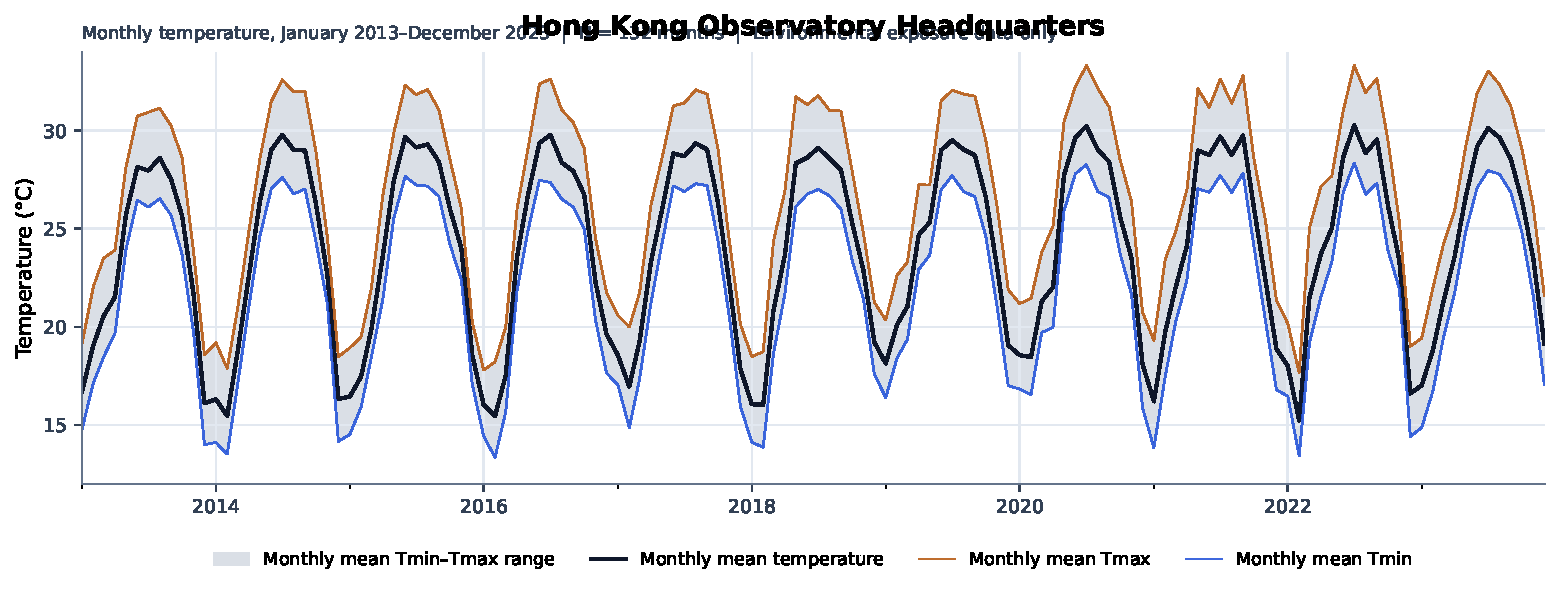
\includegraphics[width=0.95\textwidth]{../../figures/lab_meeting/monthly_temp_ribbon_2013_2023.pdf}
  \end{center}
  \vspace{-0.4em}
  \begin{center}
  \scriptsize Environmental exposure data only. Series ends December 2023 ($N=132$ months).
  \end{center}
\end{frame}

%----------------------------------------------------------------------
\begin{frame}{Table~1 structure --- two panels, two denominators}
  \textbf{Panel A. Monthly environmental exposures} \hfill
  {\footnotesize $N = 132$ months \quad HKO Headquarters}

  \vspace{0.25em}
  \scriptsize
  \begin{tabular}{@{}lrrr@{}}
    \toprule
    Variable & $N$ & Mean & SD \\
    \midrule
    Mean temperature ($^\circ$C) & 132 & 24.02 & 4.70 \\
    Mean Tmin ($^\circ$C) & 132 & 22.10 & 4.69 \\
    Mean Tmax ($^\circ$C) & 132 & 26.66 & 4.82 \\
    Hot nights (days/month) & 132 & 3.40 & 5.40 \\
    Cold days (days/month) & 132 & 1.10 & 2.55 \\
    Very hot days (days/month) & 132 & 3.19 & 5.18 \\
    \bottomrule
  \end{tabular}

  \vspace{0.55em}
  \normalsize
  \textbf{Panel B. Patient / admission characteristics} \hfill
  {\footnotesize Pending HA access --- denominator TBD}

  \vspace{0.2em}
  \footnotesize
  Requested fields (descriptive Table~1 as directed): number of patients;
  qualifying episodes; age; sex; diuretics; beta blockers; metformin;
  SGLT2 inhibitors; BMI and BMI missingness.

  \vspace{0.45em}
  \footnotesize
  Panel~A has 132 month-level observations. Panel~B will use a patient-,
  admission-, or patient-month-level denominator. I will not place both under
  one undifferentiated $N$. Medication/BMI model role depends on whether a true
  at-risk cohort exists and whether measurements precede the event.
\end{frame}

%----------------------------------------------------------------------
\begin{frame}{Analysis design to confirm}
  \begin{columns}[T]
    \begin{column}{0.56\textwidth}
      {\footnotesize\textbf{Proposed default: monthly population-rate design}}
      \vspace{0.3em}
      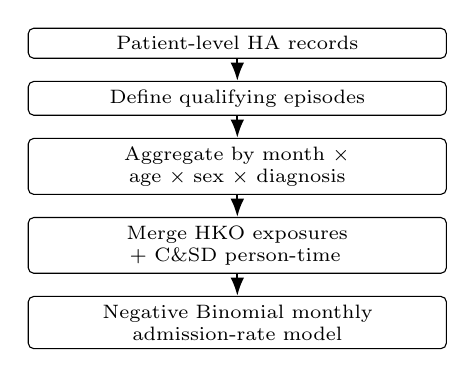
\begin{tikzpicture}[
        node distance=0.28cm,
        box/.style={draw, rounded corners=2pt, align=center,
          font=\scriptsize, inner sep=3pt, text width=5.1cm},
        arr/.style={-{Latex}, thick}
      ]
        \node[box] (a) {Patient-level HA records};
        \node[box, below=of a] (b) {Define qualifying episodes};
        \node[box, below=of b] (c) {Aggregate by month $\times$ age $\times$ sex $\times$ diagnosis};
        \node[box, below=of c] (d) {Merge HKO exposures + C\&SD person-time};
        \node[box, below=of d] (e) {Negative Binomial monthly admission-rate model};
        \draw[arr] (a) -- (b);
        \draw[arr] (b) -- (c);
        \draw[arr] (c) -- (d);
        \draw[arr] (d) -- (e);
      \end{tikzpicture}
    \end{column}
    \begin{column}{0.42\textwidth}
      {\footnotesize\textbf{Alternative, if available}}
      \vspace{0.35em}
      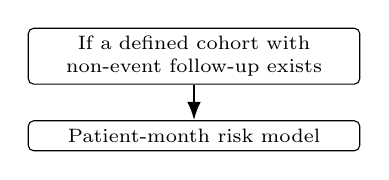
\begin{tikzpicture}[
        box/.style={draw, rounded corners=2pt, align=center,
          font=\scriptsize, inner sep=3pt, text width=4.0cm},
        arr/.style={-{Latex}, thick}
      ]
        \node[box] (f) {If a defined cohort with non-event follow-up exists};
        \node[box, below=0.45cm of f] (g) {Patient-month risk model};
        \draw[arr] (f) -- (g);
      \end{tikzpicture}

      \vspace{0.7em}
      \footnotesize
      Admissions-only extracts support
      \textbf{monthly admission counts / rates},
      not ``patient-level risk,'' until the denominator is defined.

      \vspace{0.45em}
      My proposed default: retain the monthly population-rate design unless the HA extract contains a defined at-risk cohort.
      I would appreciate confirmation.
    \end{column}
  \end{columns}
\end{frame}

%----------------------------------------------------------------------
\begin{frame}{Lag variables and proposed model ladder}
  \begin{columns}[T]
    \begin{column}{0.48\textwidth}
      \begin{center}
        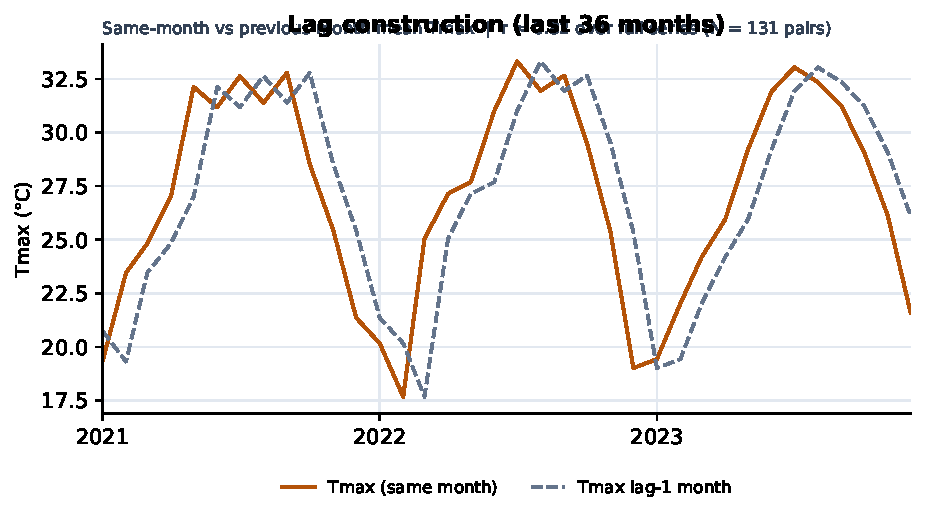
\includegraphics[width=\textwidth]{../../figures/lab_meeting/tmax_lag1_example_revised.pdf}
      \end{center}
    \end{column}
    \begin{column}{0.50\textwidth}
      \footnotesize
      \begin{itemize}
        \item Contemporaneous and lag-1 variables can both be added to the merge.
        \item Current and lag-1 Tmax are strongly correlated ($r \approx 0.82$; 131 pairs).
        \item Same-month exposure proposed as primary.
        \item Lag-1 proposed as a separate sensitivity model.
        \item Current/previous-month average may be secondary.
        \item Do not put mean, Tmin, Tmax, and all lags together in one initial model.
      \end{itemize}

      \vspace{0.35em}
      December 2012 daily HKO data exist in the raw extracts, but the processed monthly file currently starts January~2013, so January~2013 lag-1 is missing unless we extend the weather build.
      I recommend extending the weather input to December~2012.
    \end{column}
  \end{columns}

  \vspace{0.35em}
  \footnotesize
  I propose this model ladder and would welcome confirmation.
\end{frame}

%----------------------------------------------------------------------
\begin{frame}{Confirmations needed and next deliverable}
  \footnotesize
  \begin{enumerate}
    \item \textbf{DAE and row/episode definition.} What ``DAE records included'' means; whether one row = one admission episode.
    \item \textbf{Principal diagnosis, admission route, transfers, and recurrence.} Principal-only vs any position; elective vs emergency; transfer/recurrence rules.
    \item \textbf{Admissions-only dataset versus defined at-risk cohort.} This determines whether we stay with monthly population rates or move to a patient-month risk model.
    \item \textbf{Medication/BMI timing and IRB amendment.} Are fields on the approved extract? Pre-event timing? IRB update is a PI decision.
  \end{enumerate}

  \vspace{0.35em}
  \textbf{Immediate actions}
  \vspace{0.15em}
  \begin{itemize}
    \item \textbf{Bob:} wet-ink; extend weather to Dec~2012; prepare HA descriptive scripts; draft Table~1 Panel~B shell.
    \item \textbf{Roro:} clarify DAE / episode / denominator / meds-BMI fields; onboard Bob after signatures.
    \item \textbf{Hogan:} wet-ink; advise on station choice / any pollution extension timing.
    \item \textbf{Professor Bishai:} confirm design default, model ladder, covariate role, and IRB path.
  \end{itemize}

  \vspace{0.45em}
  \textbf{Next deliverable:} validated HA descriptive counts, missingness, episode
  definitions, age-specific rates, and completed Table~1. No causal claims.
\end{frame}

%======================================================================
\appendix
\begin{frame}[plain]
  \centering
  \vspace{2.2cm}
  {\Large\bfseries Appendix}\\[0.6em]
  {\small Technical detail for discussion if needed}
\end{frame}

%----------------------------------------------------------------------
\begin{frame}{A1. Provisional ICD-9 definitions}
  \footnotesize
  Coding system \textbf{confirmed ICD-9} (Roro, 12~July). Code lists remain provisional until principal-diagnosis and local HA rules are confirmed.

  \vspace{0.4em}
  \begin{tabular}{@{}llp{5.8cm}@{}}
    \toprule
    Group & Codes & Notes \\
    \midrule
    AMI & 410.x & Exclude old MI 412 \\
    Hemorrhagic stroke & 430, 431; provisionally 432.x & Sensitivity: 430--431 only \\
    Ischemic stroke & 433.x1, 434.x1, 436 & Sensitivity: with/without 436 \\
    Exclude & 412; 435.x; 438.x & Old MI; TIA; stroke sequelae \\
    \bottomrule
  \end{tabular}

  \vspace{0.5em}
  Source: \texttt{memos/data\_request\_roro.md}. ICD-10 backup retained only if needed historically.
\end{frame}

%----------------------------------------------------------------------
\begin{frame}{A2. Full HKO validation table (annual extremes)}
  \scriptsize
  Station: HKO Headquarters. Result: \textbf{33/33 MATCH} vs HKO \textit{The Year's Weather}.

  \vspace{0.3em}
  \begin{tabular}{@{}rrrr@{}}
    \toprule
    Year & Hot nights & Very hot days & Cold days \\
    \midrule
    2013 & 10 & 17 & 14 \\
    2014 & 34 & 33 & 21 \\
    2015 & 37 & 28 & 7 \\
    2016 & 36 & 38 & 21 \\
    2017 & 41 & 29 & 9 \\
    2018 & 26 & 36 & 21 \\
    2019 & 46 & 33 & 1 \\
    2020 & 50 & 47 & 11 \\
    2021 & 61 & 54 & 13 \\
    2022 & 52 & 52 & 13 \\
    2023 & 56 & 54 & 14 \\
    \bottomrule
  \end{tabular}

  \vspace{0.35em}
  Source: \texttt{outputs/tables/hko\_annual\_extremes\_validation.csv}.
\end{frame}

%----------------------------------------------------------------------
\begin{frame}{A3. Detailed data questions for Roro}
  \footnotesize
  \begin{enumerate}
    \item What does ``DAE records included'' mean in this ICD-9 extract? (I do not invent an expansion.)
    \item Is each row one admission episode, with drugs/BMI attached if available?
    \item Can principal diagnosis be distinguished from secondary diagnoses?
    \item Are elective inpatient admissions included, given no ED-to-inpatient episodes?
    \item How are inter-hospital transfers and same-patient recurrence handled?
    \item Are diuretics, beta blockers, metformin, SGLT2is, and BMI already on the approved extract?
    \item What medication and BMI measurement dates are available relative to admission?
    \item Does the extract contain non-event follow-up / a defined at-risk cohort, or admissions only?
    \item What small-cell suppression rules apply to descriptive outputs from HPC?
  \end{enumerate}
\end{frame}

%----------------------------------------------------------------------
\begin{frame}{A4. Pipeline diagram (ready for real HA merge)}
  \footnotesize
  \begin{center}
  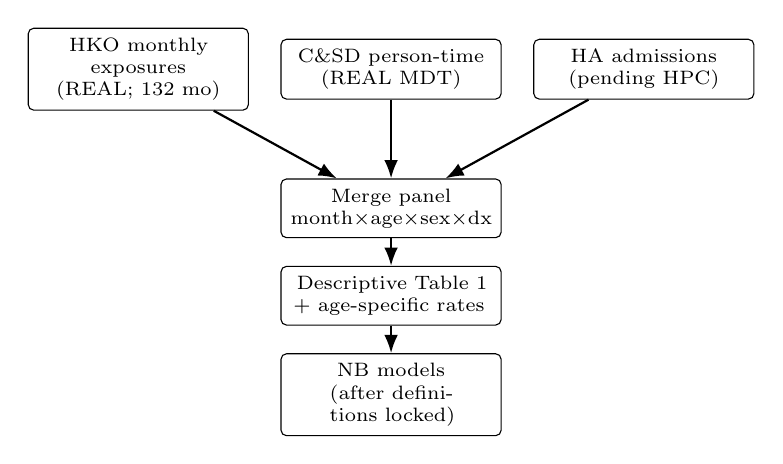
\begin{tikzpicture}[
    node distance=0.35cm and 0.4cm,
    box/.style={draw, rounded corners=2pt, align=center, font=\scriptsize,
      inner sep=3.5pt, text width=2.55cm},
    arr/.style={-{Latex}, thick}
  ]
    \node[box] (hko) {HKO monthly exposures\\(REAL; 132 mo)};
    \node[box, right=of hko] (csd) {C\&SD person-time\\(REAL MDT)};
    \node[box, right=of csd] (ha) {HA admissions\\(pending HPC)};
    \node[box, below=1.0cm of csd] (merge) {Merge panel\\month$\times$age$\times$sex$\times$dx};
    \node[box, below=of merge] (desc) {Descriptive Table~1\\+ age-specific rates};
    \node[box, below=of desc] (mod) {NB models\\(after definitions locked)};
    \draw[arr] (hko) -- (merge);
    \draw[arr] (csd) -- (merge);
    \draw[arr] (ha) -- (merge);
    \draw[arr] (merge) -- (desc);
    \draw[arr] (desc) -- (mod);
  \end{tikzpicture}
  \end{center}

  \vspace{0.4em}
  Scripts: \texttt{02\_build\_weather\_monthly.R}, \texttt{05\_build\_population\_denominators.R},
  \texttt{08b\_merge\_real\_ha\_panel.R}, \texttt{09}--\texttt{11}. Synthetic track exists only for workflow testing --- not findings.
\end{frame}

%----------------------------------------------------------------------
\begin{frame}{A5. Full Table~1 shell}
  \footnotesize
  \textbf{Panel A --- filled} ($N=132$ months; HKO Headquarters)\\[0.2em]
  Mean temp 24.02 (4.70); Tmin 22.10 (4.69); Tmax 26.66 (4.82);
  hot nights 3.40 (5.40); cold days 1.10 (2.55); very hot days 3.19 (5.18).

  \vspace{0.55em}
  \textbf{Panel B --- pending HA access}\\[0.2em]
  \begin{tabular}{@{}lp{8.6cm}@{}}
    \toprule
    Field & Status / note \\
    \midrule
    $N$ patients / episodes & Pending; denominator depends on design fork \\
    Age, sex & Requested; strata include 65--69 and 70--74 \\
    Diuretics; beta blockers & Requested descriptively; model role TBD \\
    Metformin; SGLT2 inhibitors & Requested descriptively; model role TBD \\
    BMI (+ missingness) & Requested descriptively; pre-event timing TBD \\
    \bottomrule
  \end{tabular}

  \vspace{0.4em}
  \scriptsize
  I will include these covariates descriptively as requested. Their use as model
  confounders depends on cohort structure and measurement timing.
\end{frame}

%----------------------------------------------------------------------
\begin{frame}{A6. Possible pollution and district extensions}
  \footnotesize
  \begin{itemize}
    \item \textbf{Pollution:} EPD import scripts ready; current file is a placeholder.
      Near-term priority remains temperature $\rightarrow$ AMI/stroke after HA access.
      Pollution can enter staged models after the first validated descriptive report.
    \item \textbf{District / multi-station weather:} HKO Headquarters is the primary
      station (matches official extreme-day definitions). Multi-station or district
      extensions are optional sensitivities (Hogan), not required for the first HA report.
    \item \textbf{2024 weather extension:} Optional; raw 2024 extract exists.
      Do not delay the 2013--2023 HA core.
  \end{itemize}
\end{frame}

\end{document}
